
\section{Evaluation}
\label{sec:evaluation}
We evaluate the performance of {\specula} using Amazon's EC2. We deployed the system over geo-distributed datacenters and evaluated with three workloads: a synthetic workload, TPC-C and RUBiS. The results show that our protocol can achieve about 2$\times$ speedup for low contention workload (RUBiS) and is especially beneficial (6$\times$ speedup) for workloads with low local contention and high remote contention (a payment-dominant TPC-C workload).

\subsection{Protocol variations and baselines}
We include two variations of our protocol, {\specula}-Internal and  {\specula}-External: in  {\specula}-Internal, the auto tuner can only switch between allowing speculative read or not, while it can not speculatively commit transactions;  {\specula}-External allows both speculative read and speculative commit. {\specula}-External tunes the speculation level from no speculative read (No SR), speculative read but no speculative commit (SR+SL0), SR+SL1 to SR+SL8.
 
We compare our protocol against two baseline protocols. The first one is based on ClockSI \cite{ClockSI}, a decentralized transactional protocol that provides Snapshot Isolation. The original ClockSI protocol does not support replication and we added a simple replication mechanism: when a master partition receives a prepare request, it synchronously replicates it to its replicas. The replicas then acknowledge to the transaction coordinator directly and the coordinator commits the transaction when it has received prepare from all involved partitions and their replicas. The protocol requires one and half WAN round-trip to commit a transaction. We name it as \textbf{ClockSI-Rep}.

The second baseline is designed to emulate PLANET \cite{planet}, which permits speculatively committing transaction while not allowing speculative read or pipelining speculative transactions.  The originally proposed PLANET is built on top of the MDCC protocol \cite{MDCC} and decides to speculative commit a transaction or not by a prediction model. Since it is not possible to do an apple-to-apple comparison, we emulate a simplified version of PLANET, by building it atop ClockSI-Rep and additionally allows each client to speculatively commit one transaction. 

\subsection{Experimental setup}
\label{subsec:setup}
We implemented our baseline protocol and speculative protocol using the Erlang programming language, on top of \textit{antidote}, an open-source reference platform for evaluating distributed consistency protocols \cite{antidote}.

We deployed the system in nine datacenters of Amazon EC2: Ireland(IE), Seoul(SU), Sydney(SY), Oregon(OR), Singapore(SG), North California(CA), Frankfurt(FR), Tokyo(TY) and North Virginia(VA). Each datacenter consists of three m4.large instances (2 VCPU and 8 GB of memory) and each instance holds the master replica of one partition. All DCs form a consistent hashing ring according to the order of the above list; the data of each instance is replicated by five following datacenters' corresponding servers, e.g. the data of DC CA is replicated by DCs FR, TY, VA, IE and SU. We interleave DCs from nearby regions in the hashing, so that each replication group has similar maximal latency, as shown in table \ref{tab:latency}.

We locate a workload stressor in each instance that issues transactions to local transaction coordinators. If a transaction is aborted, the client retries it until it gets committed. Each experiment is run for three times. We discard the aggregate results of the first twenty seconds and show the average value (deviation is low).

\begin{table*}
\small
\begin{center}
  \begin{tabular}{l |  l | l | l| l | l | l| l| l |l } 
     & IE & SU& SY& OR & SG & CA &  FR & TY & VA  \\ \hline
  \textbf{Max latency (replicas)} & 334(SG) & 267(FR) & 321(FR) & 160(SG)  & 337(IE) & 167(FR) & 321(SY)& 212(IE)  &  226(SY)  \\   \hline
  \textbf{Max latency (all)} &  334(SG) &  267(FR) & 321(FR)  & 163(SY) & 337(IE) & 175(SG) & 324(SG)  & 233(FR)  & 226(SY) \\ \hline
  \end{tabular}
\end{center}
\caption{Maximal mean latency of a DC to its replicas and to all other DC}
\label{tab:latency}
\end{table*}


\subsection{Synthetic workloads}
Our evaluation starts with synthetic workloads. The synthetic workloads simulate idealistic non-interactive workloads, where each thread issues a new transaction as soon as the previous one is committed (or speculative committed). The tunable speculation levels are the following, from conservative to aggressive: no speculative read (SR for short) and speculation length zero (SL0), SR and SL0, SR and SL1, ..., SR and SL8. We first compare {\specula}-Strong and {\specula}-Tuning with the baselines, then via a separate experiment we compare the effectiveness of auto-tuning method with static configurations.

\paragraph{Transaction and data access} A transaction reads 10 keys then updates them. 90\% of key access goes to a small range of each data partition, a.k.a hotspot, and we adjust the size of hotspot to control contention rate. Each data partition has two million keys, of which one million are only accessible by local-initiated transactions and the other are only accessible by remote transactions. This allows adjusting local contention level (i.e. the contention level when a local transaction performs local certification) without affecting remote conflict level. In the following experiments, we denote 30000 keys for the size of local hotspot size as \textbf{low local contention} and 1000 keys as \textbf{high local contention}; according, 15000 keys for a remote hotspot is named \textbf{low remote contention} and 500 for \textbf{high remote contention}. The following workloads use high data locality: 80\% access goes to local master partitions, while 20\% goes to slave data partitions replicated locally.

\begin{figure*}
\centering
\def\svgwidth{0.98\columnwidth}
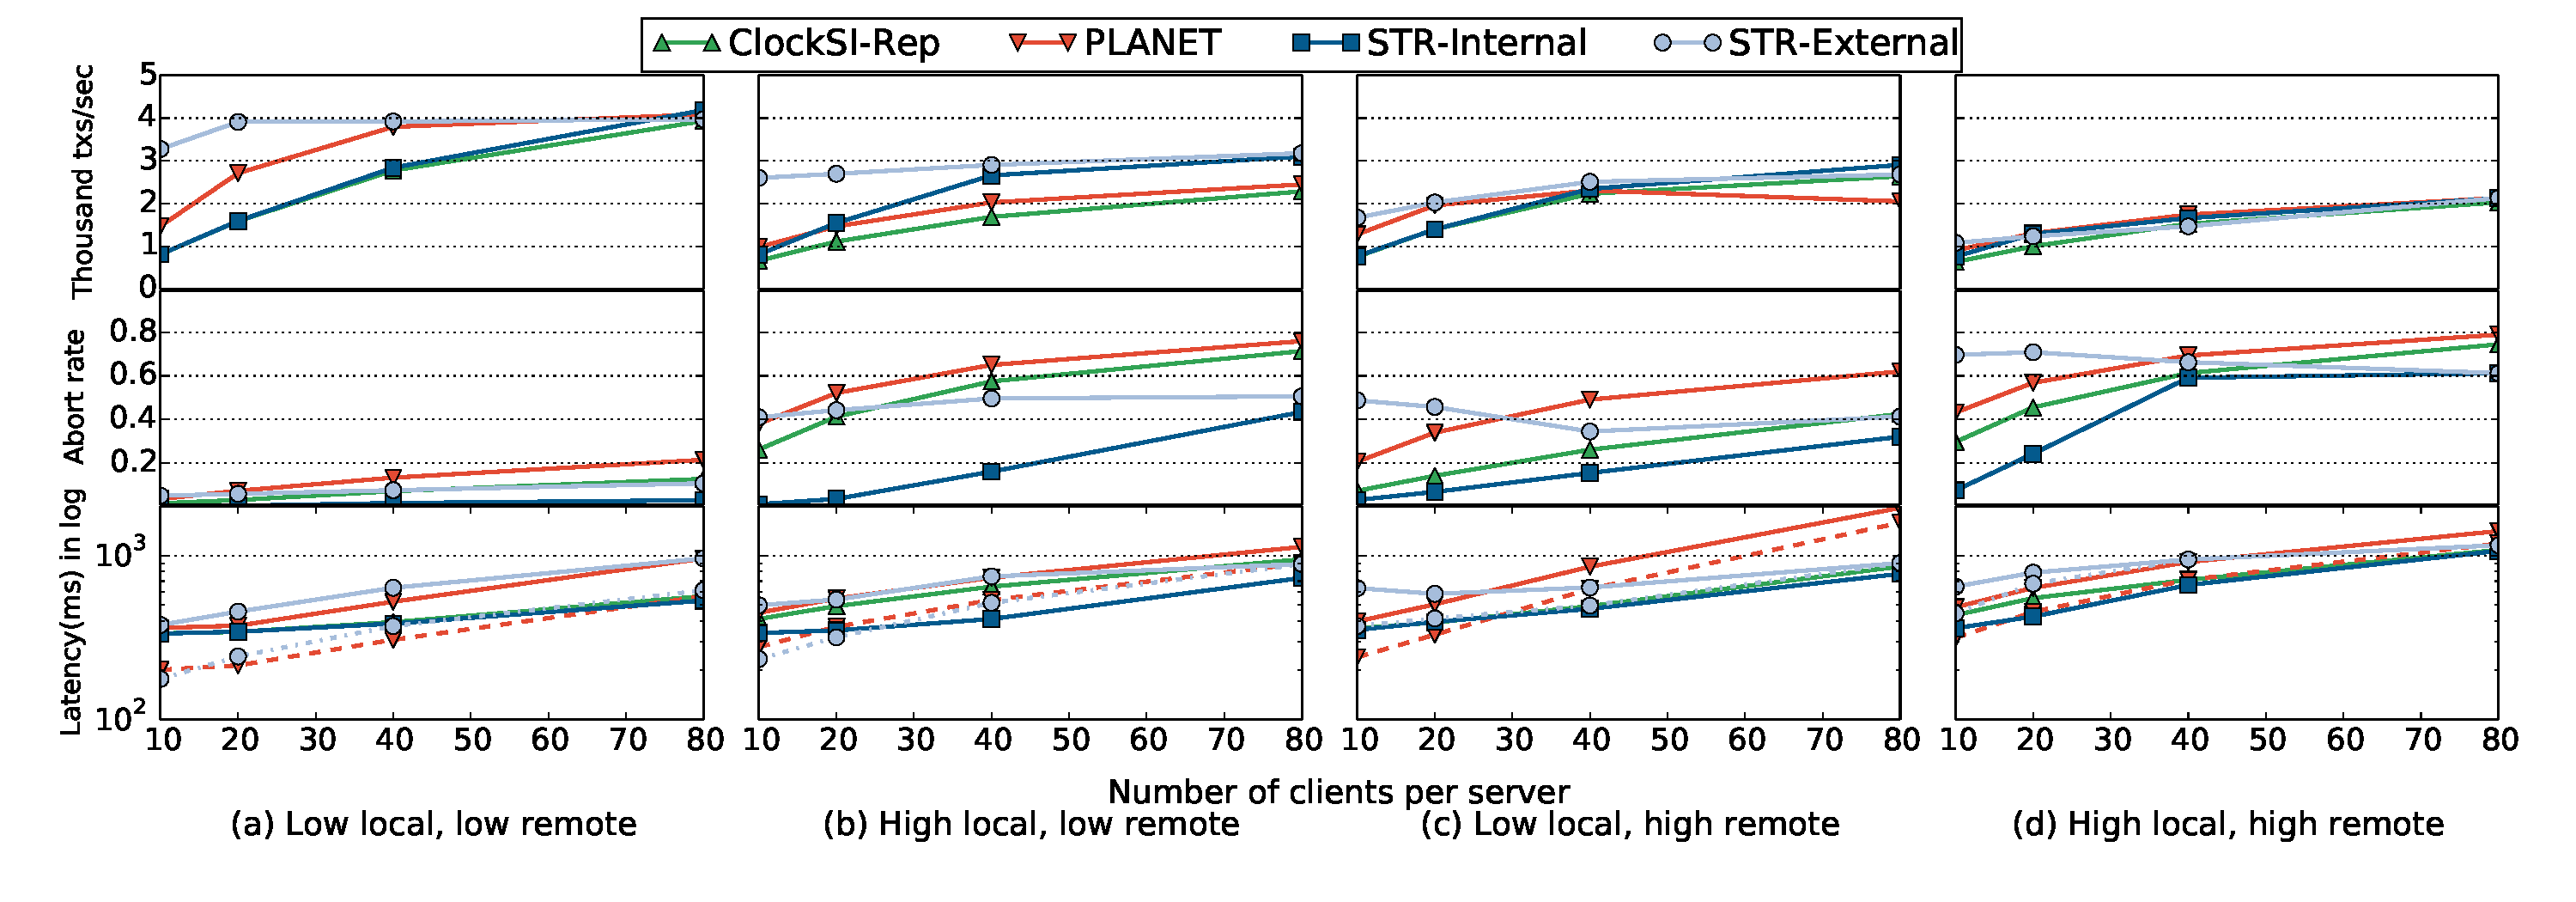
\includegraphics[scale=0.35]{figures/micro}
\hspace{-10mm}
\caption{\textit{Performance of different protocols under four levels of contention.} \textit{Low local, low remote} denotes low local contention and low remote contention, and so forth. For latency, solid lines denote final latency and dashed lines are the perceived latency.}
\label{fig:micro_conflict}
\end{figure*}


\begin{figure}[t]
\centering
\def\svgwidth{0.98\columnwidth}
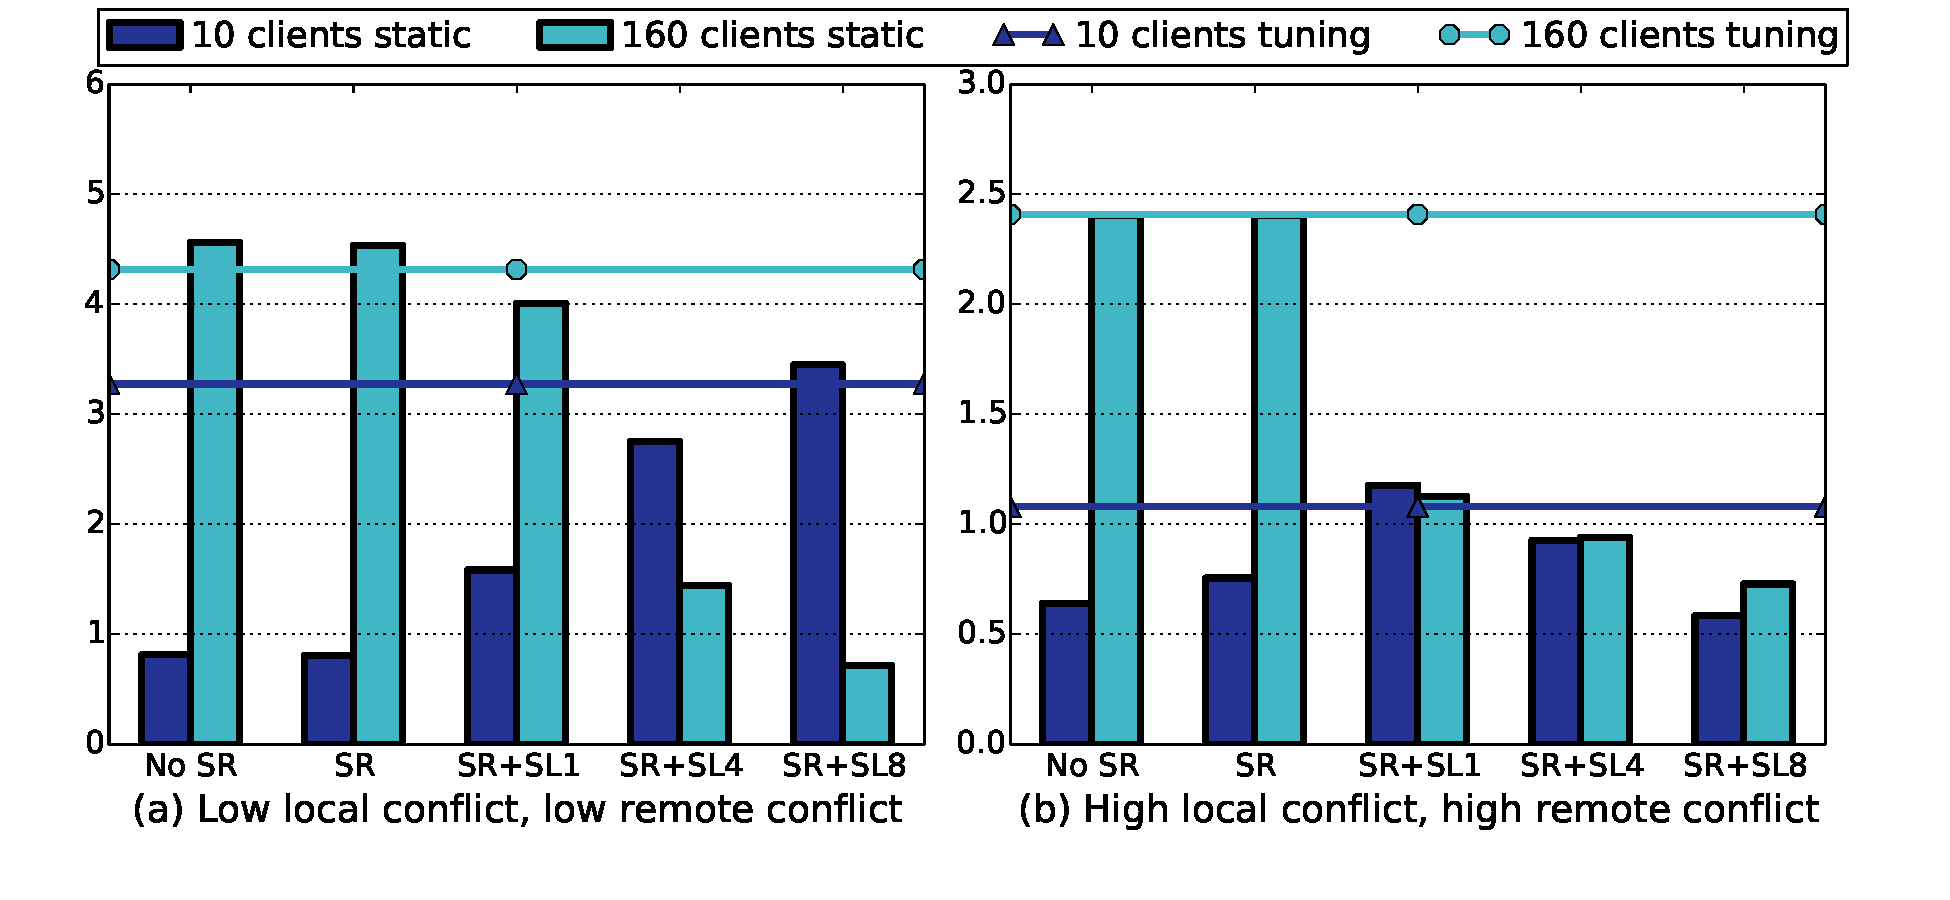
\includegraphics[scale = 0.28]{figures/tuning}
\vspace{-7mm}
\caption{\footnotesize The throughput of tuning versus static configuration}
\label{fig:tuning}
\end{figure}

\paragraph{Performance under different contentions} In this set of experiments, we vary contention levels and system load, i.e. number of clients, to examine the performance of ClockSI-Rep, PLANET, {\specula}-Internal and {\specula}-External. As mentioned, both variations of {\specula} has an automatic tuning method. 

For low contention workload (\ref{fig:micro}a), both PLANET and {\specula}-External achieve good speedup, because they all allow speculatively committing transactions so clients can perform more work. Though, the key difference is that {\specula}-External supports pipelining multiple transactions, so it can achieve high throughput with much fewer clients than PLANET. The speedup reduces when the system gets more saturated. {\specula}-Internal has very little speedup, as this workload has low contention so speculative read rarely occurs. Still, {\specula}-Internal has much lower conflict rate than both ClockSI-Rep and PLANET due to the use of PreciseClock.

Figure \ref{fig:micro}b shows the throughput of different protocols in a workload with high local contention and low remote contention. This workload is beneficial for {\specula}-Internal and {\specula}-External, as they allow speculative read to avoid getting blocked when trying to read pre-commit records, and transactions being speculatively-read are likely to commit due to low remote contention. On the other hand, because PLANET does permit not speculative read, it achieves littler performance gain. The effect of speculative read is directly reflected in latency: the latency of PLANET and ClockSI-Rep considerably increase compared with figure \ref{fig:tuning}a, while the latency of {\specula}-Internal and {\specula}-External are not affected due to speculative read.

Next, we examine workloads with high remote contention, which is unfavorable for speculation. As figure \ref{fig:micro}c shows, PLANET has large performance penalty and large latency, as speculative commit often fails due to high remote contention. Although {\specula}-Strong also allows speculative commit, thanks to the auto-tuning algorithm, it get good throughput despite the number of clients. The performance of STR-Internal are similar to ClockSI-Rep again (as in figure \ref{fig:micro}), due to having low local contention. The last workload combines both high local contention and high remote contention, but {\specula}-External and {\specula}-Internal still remain stable throughput due to auto-tuning. Nevertheless, PLANET achieves higher throughput than in figure \ref{fig:micro}c, because high local contention causes transactions to be blocked and perform less speculative commit.

\paragraph{Automatic tuning v.s. static configurations} This experiment compares the throughput of 10 clients and 160 clients per server, using either automatic tuning or static tuning, e.g. not allowing speculative read (No SR), allowing speculative read and speculative commit with length one (SR+SL1). We picked two extreme workloads, one with low local and remote contention, and one with high contention for both. As shown in figure \ref{fig:tuning}, the levels of speculation to achieve optimal throughput vary for different numbers of clients and different contention, which is hard to predict in advance. This is indeed what we observed when experimenting different speculation levels and motivated us to design the automatic tuning method. More importantly, as can be seen in the figure, the curve of speculation level to throughput is convex, i.e. if a speculation level gives local maximal throughput, this is guaranteed to be a global maximum throughput. This observation drove us to design the automatic tuning method as a simple hill climbing algorithm \cite{hillclimbing}, which is simple and fast yet can reach throughput close to the optimal throughput (figure \ref{fig:tuning}).

\iffalse
\begin{figure}[t]
\centering
\begin{subfigure}[t!]{0.494\linewidth}
\def\svgwidth{0.95\columnwidth}
\hspace{-3mm}
\centering 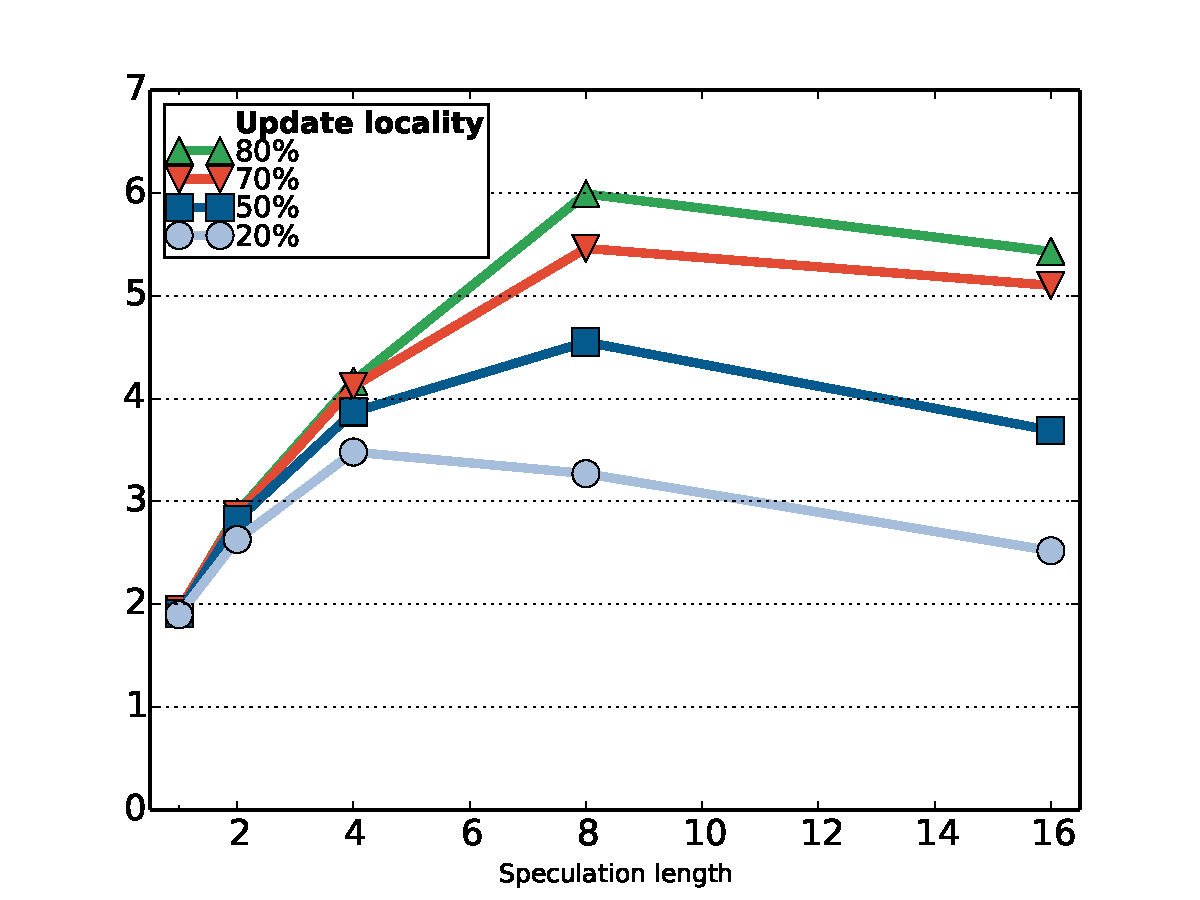
\includegraphics[scale = 0.21]{figures/updatelocality}
\caption{\footnotesize Different update locality}
\label{fig:remote:a}
\end{subfigure}
\begin{subfigure}[t!]{0.494\linewidth}
\vspace{1mm}
\def\svgwidth{0.95\columnwidth}
\centering 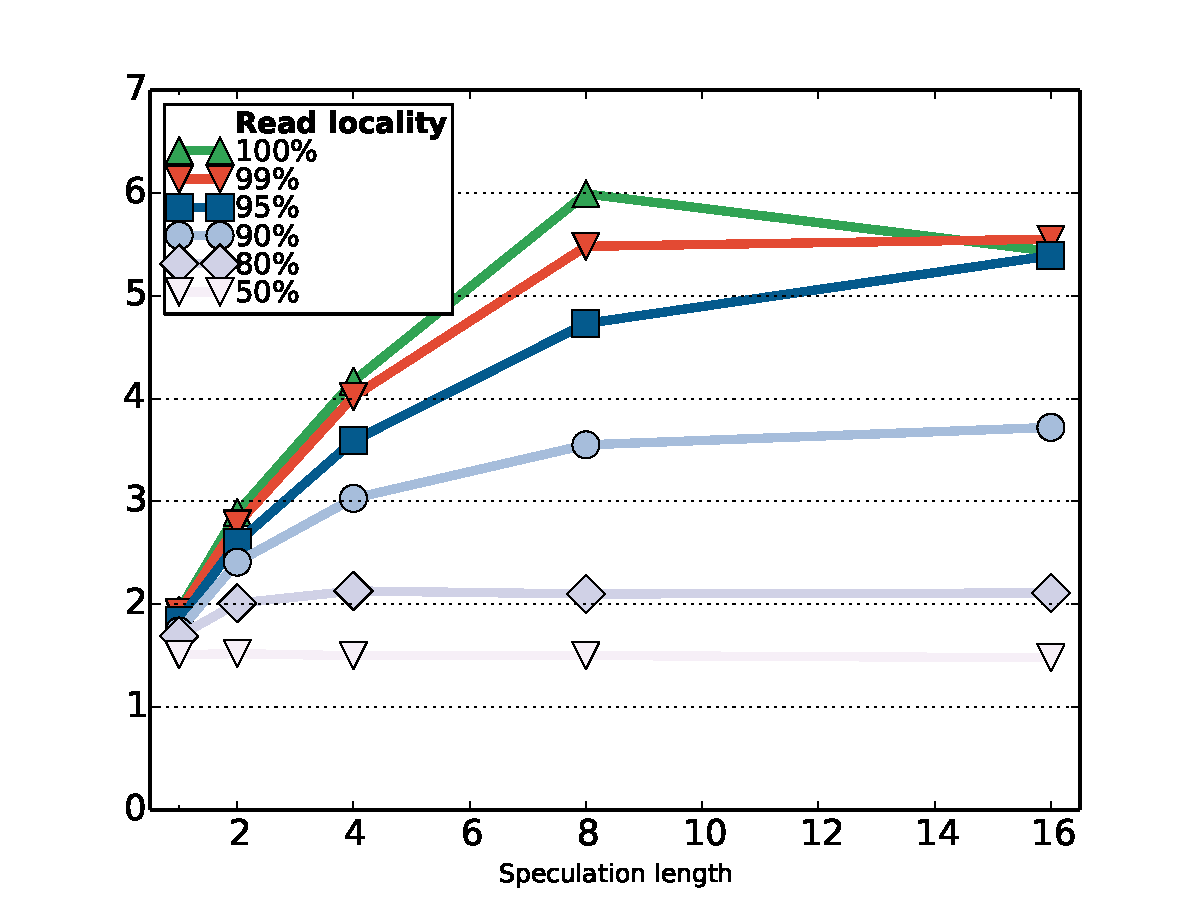
\includegraphics[scale = 0.212]{figures/readlocality}%Remotereadremoteread
\vspace{-1mm}
\caption{\footnotesize Different read locality}
\label{fig:remote:b}
\end{subfigure}
\caption{Results of the protocol with different update locality and read locality.}
\label{fig:micro_conflict}
\end{figure}

\paragraph{Locality} In this experiment we vary update locality and read locality. Contention rate is fixed to be low for both local contention and remote contention.

In the first test, we vary update locality while still keep 100\% read locality. The three numbers of each legend denote respectively the probability for a transaction to access its local master partition, local DC replicated partitions and remote DC partitions. Figure \ref{fig:remote:a} shows that lower update locality causes higher abort rate that leads to lower throughput. Figure \ref{fig:remote:b} presents the speedup of the speculative protocol compared with the baseline with different remote read probability, i.e. read locality. Intuitively, with lower read locality, a transaction takes longer time to execute before certification, so speedup should be reduced. With less than 5\% of remote read, the speculative protocol achieves similar speedup, and even when there are 50\% of remote read, we still have about 1.5$\times$ speedup.

\fi

\paragraph{Precise clock} 


%Reading a key that is not replicated locally causes large latency, which makes it difficult to examine the benefit of speculation. So for most of the experiments, a transaction only accesses keys replicated in local datacenter. We dedicate a separate experiment to examine the effect of remote read on throughput.

\subsection{Macro benchmark}
In the following experiments, we evaluate the performance of \specula with realistic interactive workloads, namely TPC-C\cite{tpcc} and RUBiS \cite{rubis}. A dramatic of these workloads with the previous synthetic workloads are: (i) these interactive workloads typically assume large number of clients, and (ii) each client only occasionally issues operation, rather than injecting operation as fast as possible as in the synthetic workloads. Therefore, for these experiments we load the system with large number of clients and we apply the specified \textit{think time} between a client's operations (for TPC-C we also apply the \textit{key time}). For these workloads, we set the speculation length as four, which usually gives good speedup according to the synthetic workload.


\begin{figure*}
\centering
\begin{minipage}{.73\textwidth}
\hspace{-5mm}
\centering
  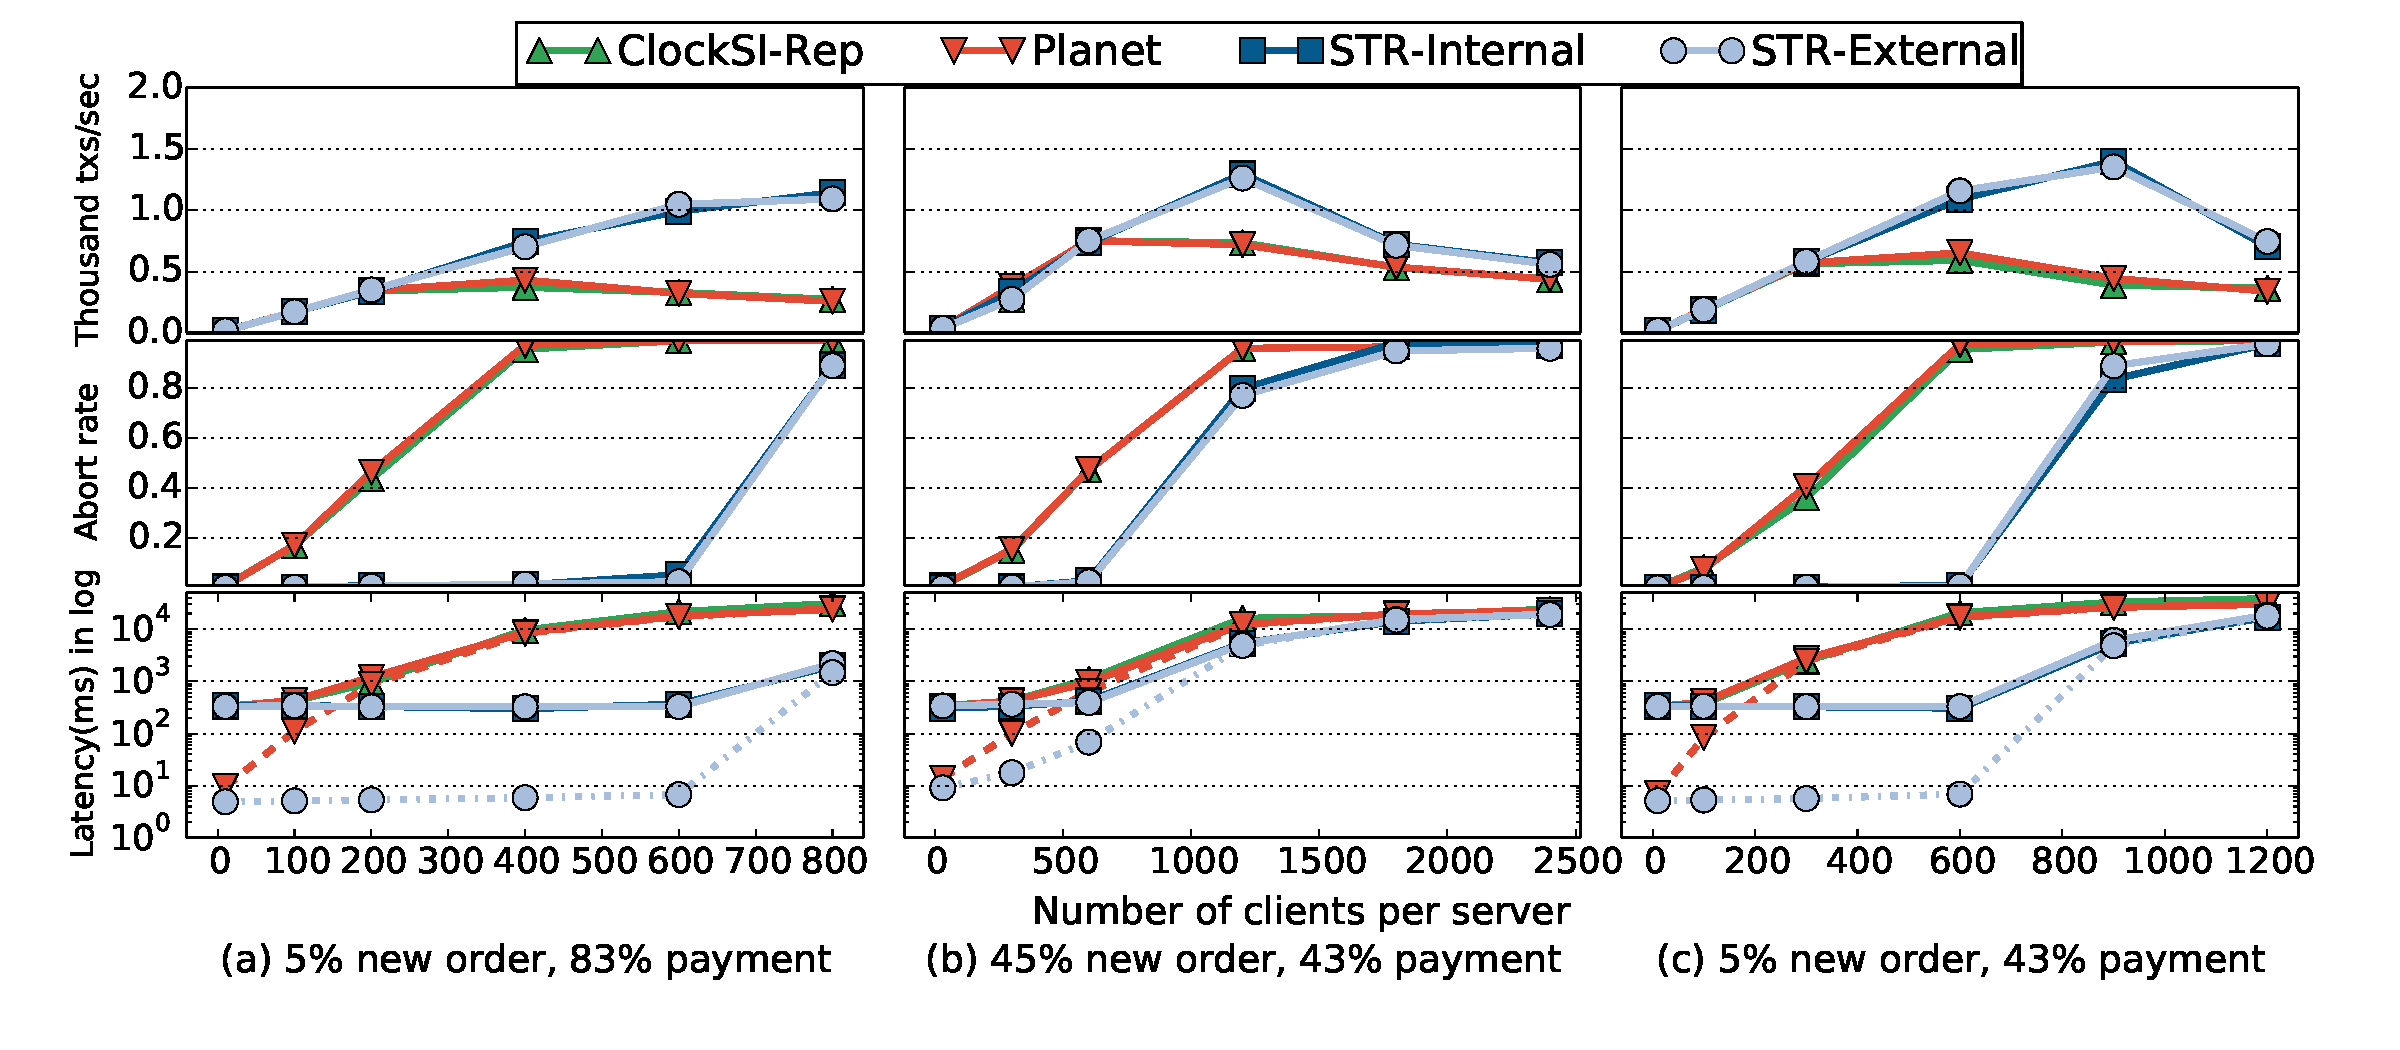
\includegraphics[scale=0.31]{figures/tpcc}
  \caption{RUBiS throughput}
  \label{fig:tpcc_result}
\end{minipage}
\begin{minipage}{.25\textwidth}
\centering
  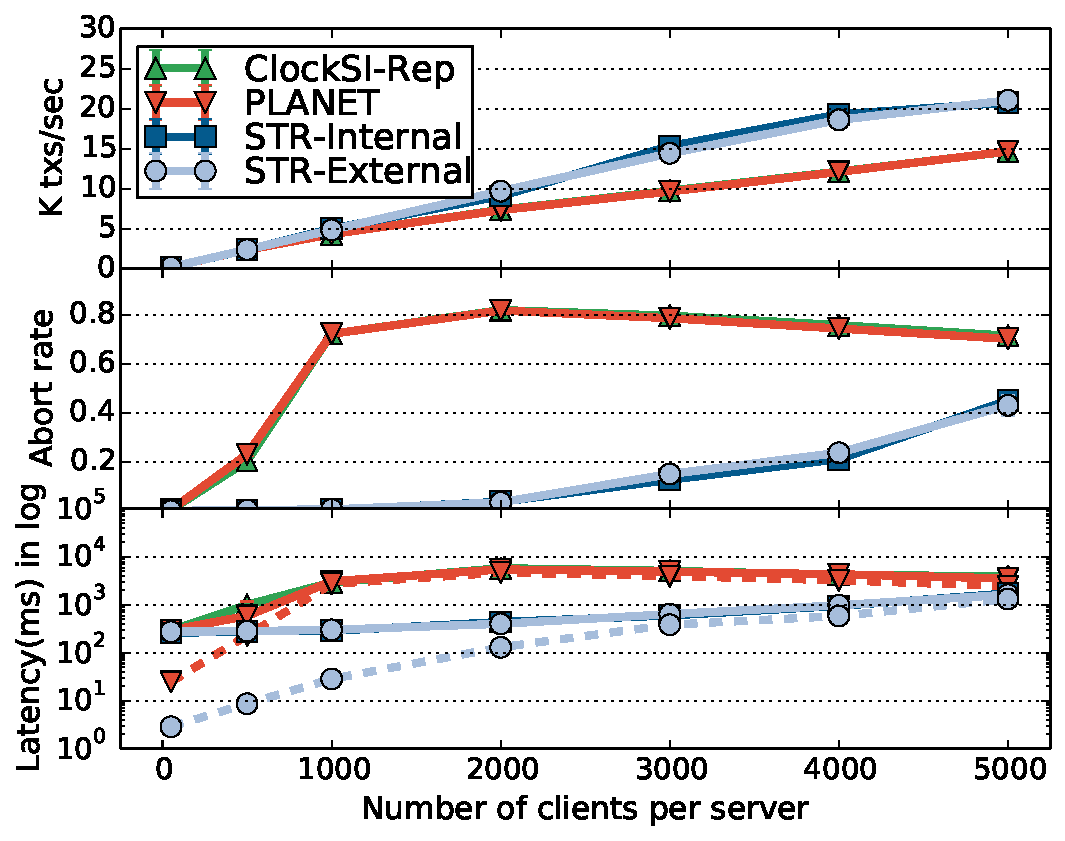
\includegraphics[scale=0.27]{figures/rubislatencywarehouse}
  \caption{RUBiS throughput}
  \label{fig:rubis}
\end{minipage}
\end{figure*}

\iffalse
\begin{table}
\small
\begin{center}
  \begin{tabular}{ l | l | l } 
    &  \scriptsize \textbf{Read-dominant} & \scriptsize \textbf{Write-dominant} \\ \hline
  \scriptsize \textbf{Payment-intensive} & \scriptsize 1\%, 9\%, 90\% &  \scriptsize 10\%, 80\%, 10\% \\
    & \scriptsize  (TPC-C PR)  &  \scriptsize (TPC-C PW) \\ \hline
  \scriptsize \textbf{New-order-intensive}  & \scriptsize 9\%, 1\%, 90\% & \scriptsize 80\%, 10\%, 10\%\\
    & \scriptsize (TPC-C NR)  &  \scriptsize (TPC-C NW) \\ \hline
  \end{tabular}
\end{center}
\caption{\textit{The ratios for new-order, payment and order-status transactions of different TPC-C workloads.} TPC-C PR means the workload is payment-intensive and read-dominant.}
\label{tab:workload}
\end{table}
\fi

\subsubsection{TPC-C}
TPC-C \cite{tpcc} models the workload of an online shopping system. We use TPC-C to examine how our speculative protocol performs under its highly skewed access. We implemented three TPC-C transactions: payment, new-order and order-status. Payment  updates the balance of a warehouse, the balance of a district from that warehouse and the balance of a customer; new-oder  updates a district and modifies the stocks for 5-15 items, and order-status is a read-only transaction. New-order  has medium local and remote conflict rate, while payment  has extremely high local contention, but very low remote contention. The locality of each transactions are as follows: new-order transactions always update local warehouses and districts, but when choosing each stock to update, it has 80\% chance to access stocks belonging to local master partition (instead of 99\%) and 20\% to access stocks belonging to local slave partitions; payment transactions update local warehouse balance and local districts balance but updates a local customer balance with 10\% probability. Overall, both types of transactions do remote certification with 90\% probability. We experiment with three workload mixes according to the specification: 5\% new-order, 83\% payment and 12\% order-status (TPC-C A); 5\% new-order, 43\% payment and 43\% order-status (TPC-C A) and 45\% new-order, 43\% payment and 12\% order-status (TPC-C C). Last but not least, we add TPC-C's think time and key time, so roughly a new-order transaction `sleeps' more than 20 seconds, while payment and order-status transactions sleep about 10 seconds.

Figure \ref{fig:tpcc:a}, \ref{fig:tpcc:b} and \ref{fig:tpcc:c} show the speedup, latency (in logarithm) and abort rate comparing \specula and the baseline, varying the total number of clients, for three workloads. As each workload contains large portion of payment transactions and payment has very high local contention, the baseline is highly contented and unable to achieve higher throughput with more loads. On the contrary, \specula is able to achieve good speedup in all workloads, especially for TPC-C A where there is very high contention, we achieve 6$\times$ speedup.

\iffalse
\begin{figure*}
\centering
\begin{minipage}{.32\textwidth}
  \centering
  \vspace{-3mm}
  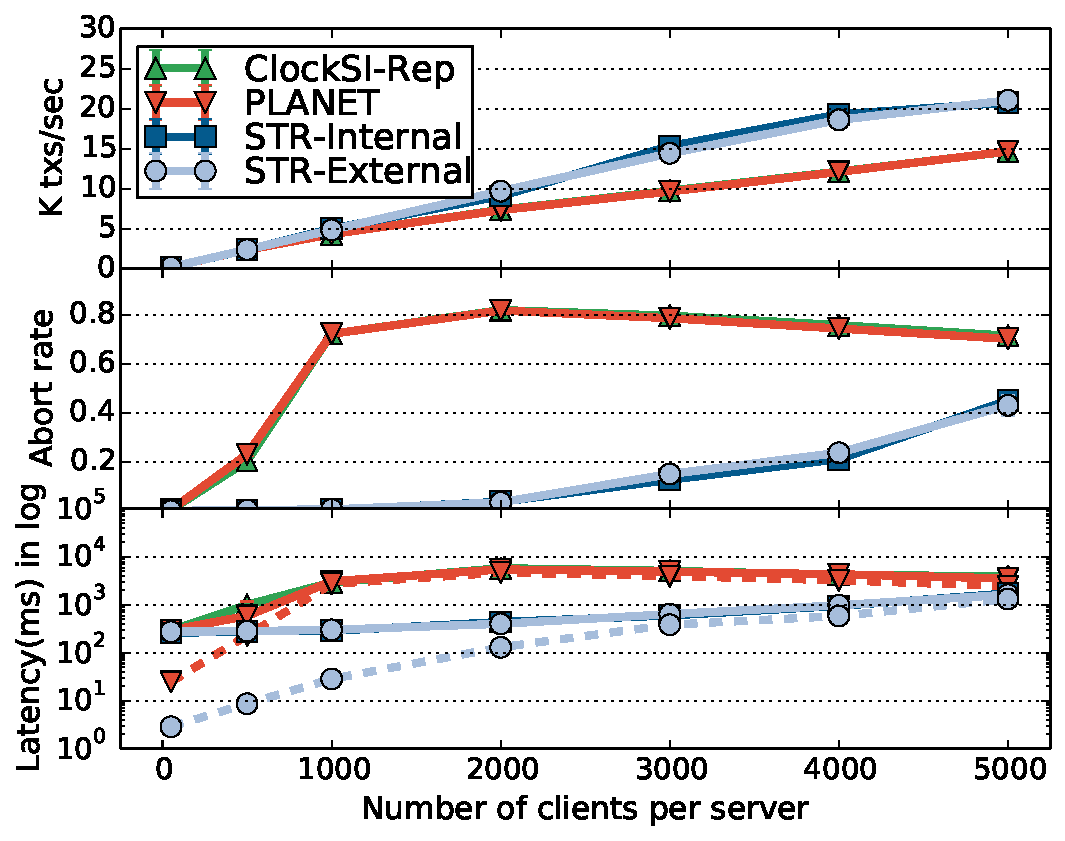
\includegraphics[scale=0.27]{figures/rubislatencywarehouse}
  \caption{Throughput of RUBiS workloads}
  \label{fig:rubis}
\end{minipage}
\begin{minipage}{.64\textwidth}
%\vspace{0mm}
  \centering
    \begin{subfigure}{0.48\linewidth}
    \def\svgwidth{0.95\columnwidth}
    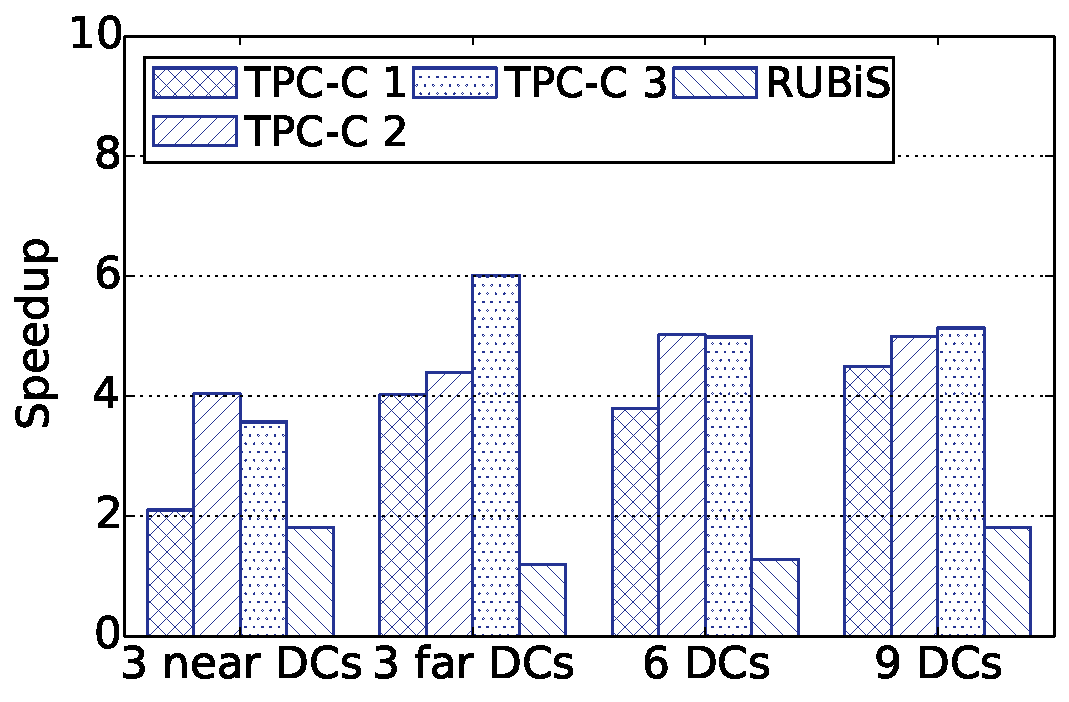
\includegraphics[scale=0.27]{figures/scale_dc}
%\vspace{-7mm}
    %\vspace{-6mm}
    \caption{\footnotesize Speedup varying num of DCs}
    %\vspace{-10mm}
    \label{fig:scale:dc}
   \end{subfigure}
%\vspace{-2mm}
  \caption{Speedup varying number of DCs and replication factors}
  \label{fig:rubis}
  
\end{minipage}
\end{figure*}

\begin{figure}
\centering
  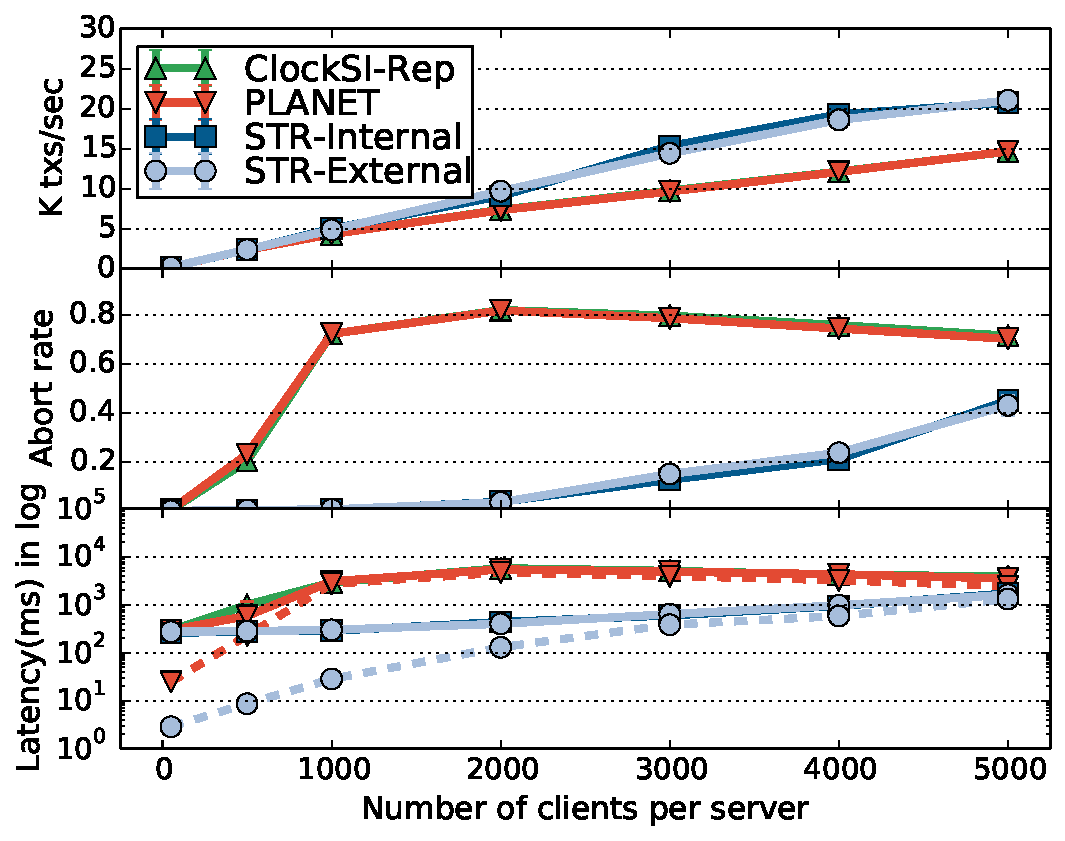
\includegraphics[scale=0.27]{figures/rubislatencywarehouse}
  \caption{Throughput of RUBiS workloads}
  \label{fig:rubis}
%\vspace{0mm}
\end{figure}
\fi

\subsection{RUBiS}
RUBiS \cite{rubis} models an online bidding system. It defines 26 user interactions, ranging from browsing all item categories, browsing user information to putting bids etc. Of all the interactions, there are five update transactions: store bid, store buy now, store comment, register item and register user, which has relatively low contention rate. We implement our own version of RUBiS with the following modification: (1) the original RUBiS benchmark workload interact with the backend server through web interface. We did not implement that. (2) RUBiS is not designed for partial replication. In our case, we horizontally partition database tables across data partitions, so that each data partition contains an equal portion of data of each table. (3) due to the assumption of full replication, many RUBiS insertion operations obtain their keys by incrementing a global table counter, so that keys are unique. Instead, for each partition we maintain a local counter for each of its table and modify the unique key generation to produce the key as a pair of partition id and the local counter, as studied in \cite{cecchet2008middleware}. We use RUBiS's 15\% update default workload.

As figure \ref{fig:rubis} shows, \specula greatly reduces the abort rate, since some RUBiS transactions (e.g. register item) present very high local contention. On the other hand, we can not achieve very high speedup, because RUBiS has lots of read-only transactions and other update transactions, rather than register item, has relatively low conflict rate. An interesting phenomena is that, with more clients, RUBiS's abort rate and latency slightly decreases. This is because in RUBiS, the more clients, the more diversed each client's access pattern is, which eventually causing less abort.
\iffalse
\subsection{Scalability}

\begin{table}
\small
\begin{center}
  \begin{tabular}{ l | l | l | l | l } 
    &  \scriptsize \textbf{3 near DCs} & \scriptsize \textbf{3 far DCs}& \scriptsize \textbf{6 DCs} & \scriptsize \textbf{9Dcs} \\ \hline
  \scriptsize \textbf{TPC-C A} & \scriptsize 3.6 &  \scriptsize  6 & \scriptsize  5 &  \scriptsize 5.1 \\ \hline
    \scriptsize \textbf{TPC-C B}  &  \scriptsize 4 & \scriptsize 4.4  & \scriptsize 5 & \scriptsize 5 \\ \hline
    \scriptsize  \textbf{TPC-C C}  &  \scriptsize 2 & \scriptsize 4  & \scriptsize 3.8 & \scriptsize 4.5 \\ \hline
   \scriptsize \textbf{RUBiS}  & \scriptsize 1.8 & \scriptsize 1.2 & \scriptsize 1.3 & \scriptsize 1.8 \\ \hline
  \end{tabular}
\end{center}
\caption{\textit{Speedup for four workloads varying the number of DCs.}}
\label{tab:speedup}
\end{table}

We test the scalability of our protocol with this last set of experiments. We vary the number of datacenters, while keeping the replication factor as two third of the number of datacenters, e.g. two for three DCs, four for six DCs and six for nine DCs. The number of threads to use is taken proportionally according to the number of clients in the above experiments where we get the best speedup. Three nearby datacenters are the three datacenters with farthest latency being 81ms. On the other hand, three faraway DCs, six DCs and nine DCs all have about 300ms of max latency. We can see that 

 so the speedups are almost the same for all workloads for these setups, as in \ref{fig:scale:rep}. However, comparing the results of three near DCs and three far DCs, note that the speedup for all workloads are higher for the three far DCs setup except for the workload TPC-C NW. Essentially, when there is low remote contention, speculation can bring larger benefit when network latency is larger. However, when there is high remote contention, larger network latency means a transaction takes longer time to commit, thus is more vulnerable to abort, which is detrimental to speculation.
 \fi
